% Compile with: pdflatex advisor_overview && pdflatex advisor_overview
% (twice so \pageref works; no bibtex needed)
\documentclass[10pt,aspectratio=169]{beamer}

\usetheme{metropolis}
\usepackage{booktabs}
\usepackage{tikz}
\usetikzlibrary{arrows.meta,positioning,calc,fit,backgrounds,shapes.geometric}
\usepackage{xcolor}
\definecolor{ours}{HTML}{2E7D32}
\definecolor{accent}{HTML}{C62828}
\definecolor{soft}{HTML}{777777}

\title{taxonomy\_agent}
\subtitle{An Orchestrator--Judge Agent for Taxonomy Discovery}
\author{Quang Minh Nguyen}
\institute{KAIST}
\date{EMNLP 2026 System Demonstrations draft}

\begin{document}
\maketitle

% --------------------------------------------------------------
\begin{frame}{Problem}
  \begin{itemize}
    \item Many applied NLP workflows start with a labelled taxonomy:
          annotation guidelines, qualitative-research codebooks,
          dashboard schemas, moderation policies.
    \item Producing one means reading hundreds of docs, drafting
          categories, arguing, iterating. Slow, expensive, brittle.
    \item LLMs can replace much of that labour — but published
          pipelines lump the proposer and the labeller into a single
          agent that can hallucinate and force its own labels.
  \end{itemize}
  \vspace{1em}
  \textbf{Our question:} can structural choices about \emph{how} the
  proposer and the labeller interact give us a cheap, honest discovery
  system?
\end{frame}

% --------------------------------------------------------------
\begin{frame}{Two structural commitments}
  \begin{enumerate}
    \item \textbf{Typed dispatcher} with \emph{validate-before-mutate}
          and \emph{per-op failure isolation}.
          \begin{itemize}
            \item Six taxonomy verbs (\textsc{add}/\textsc{rename}/
                  \textsc{edit}/\textsc{merge}/\textsc{split}/
                  \textsc{drop}).
            \item A malformed edit returns the unchanged taxonomy
                  plus a log entry the orchestrator reads next step.
                  No silent corruption.
          \end{itemize}
    \item \textbf{Stateless judge LLM.}
          \begin{itemize}
            \item Labels each item against the current taxonomy from
                  item text alone.
            \item Never sees the orchestrator's tool-call history or
                  prior label assignments.
            \item Runs on the cheap model and is called once per
                  item — cost is linear in the corpus.
          \end{itemize}
  \end{enumerate}
\end{frame}

% --------------------------------------------------------------
\begin{frame}{Architecture}
  \centering
  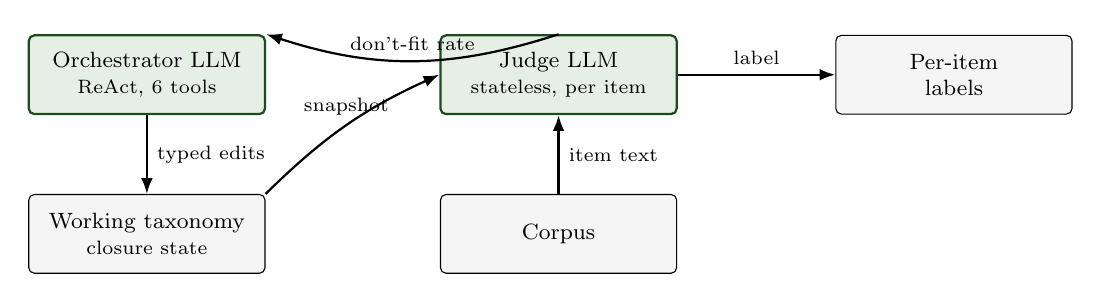
\begin{tikzpicture}[
    node distance=14mm,
    box/.style={rectangle, draw, rounded corners=2pt, minimum width=30mm,
                minimum height=10mm, align=center, font=\footnotesize},
    light/.style={box, fill=gray!8},
    ours/.style={box, fill=ours!12, draw=ours!60!black, thick},
    arrow/.style={-{Latex[length=2mm]}, thick},
  ]
    \node[ours] (orch) {Orchestrator LLM\\\scriptsize ReAct, 6 tools};
    \node[ours, right=22mm of orch] (judge) {Judge LLM\\\scriptsize stateless, per item};
    \node[light, below=10mm of orch] (tax) {Working taxonomy\\\scriptsize closure state};
    \node[light, below=10mm of judge] (corpus) {Corpus};
    \node[light, right=20mm of judge] (out) {Per-item\\labels};

    \draw[arrow] (orch.south) -- node[right,font=\scriptsize]{typed edits} (tax.north);
    \draw[arrow] (tax.north east) to[bend left=10] node[above,font=\scriptsize]{snapshot} (judge.west);
    \draw[arrow] (corpus.north) -- node[right,font=\scriptsize]{item text} (judge.south);
    \draw[arrow] (judge.east) -- node[above,font=\scriptsize]{label} (out.west);
    \draw[arrow] (judge.north) to[bend left=18] node[above,font=\scriptsize]{don't-fit rate} (orch.north east);
  \end{tikzpicture}

  \vspace{0.5em}
  \footnotesize
  Judge is read-only on the taxonomy and re-derives every label from item text. \\
  Orchestrator cannot force a label past it.
\end{frame}

% --------------------------------------------------------------
\begin{frame}{20 Newsgroups results (5 seeds, install default)}
  \centering
  \footnotesize
  \begin{tabular}{lccc}
    \toprule
    & NMI $\uparrow$ & ARI $\uparrow$ & Cost (USD) \\
    \midrule
    \textcolor{ours}{\textbf{taxonomy\_agent (cheap pair, both DeepSeek-v4-Flash)}}
      & \textbf{0.740 $\pm$ .055} & \textbf{0.489 $\pm$ .085} & 0.17 \\
    taxonomy\_agent (Sonnet orchestrator, 3 seeds)
      & 0.656 $\pm$ .012 & 0.336 $\pm$ .035 & 1.86 \\
    \midrule
    topicgpt \emph{(Pham et al.\ NAACL 2024, official code)}
      & 0.606 $\pm$ .026 & 0.297 $\pm$ .047 & 0.12 \\
    embed-cluster-LLM (TnT-LLM family, our pipeline)
      & 0.488 $\pm$ .013 & 0.243 $\pm$ .010 & 0.02 \\
    single-shot LLM
      & 0.345 $\pm$ .056 & 0.101 $\pm$ .041 & 0.02 \\
    iterative-proposal LLM
      & 0.222 $\pm$ .128 & 0.043 $\pm$ .043 & 0.03 \\
    Brady--Islam 2025 (their code via OpenRouter)
      & 0.164 $\pm$ .092 & 0.022 $\pm$ .002 & $<$0.01 \\
    BERTopic, LDA
      & $\leq$ 0.16 & $\leq$ 0.02 & 0.00 \\
    \bottomrule
  \end{tabular}
  \vspace{0.7em}

  \begin{itemize}\itemsep0.1em
    \item Cheap pair leads strongest LLM baseline (TopicGPT) by
          \textbf{1.22$\times$} NMI / \textbf{1.65$\times$} ARI.
    \item Sonnet at 11$\times$ the cost does not improve over the
          cheap pair $\Rightarrow$ orchestrator quality is not the
          bottleneck.
  \end{itemize}
\end{frame}

% --------------------------------------------------------------
\begin{frame}{CoT-Pattern results (149 items, 5 failure modes)}
  \centering
  \footnotesize
  \begin{tabular}{lcc}
    \toprule
    & NMI $\uparrow$ & Purity $\uparrow$ \\
    \midrule
    \textcolor{ours}{\textbf{taxonomy\_agent (cheap pair, 3 seeds)}}
      & \textbf{0.944 $\pm$ .081} & \textbf{0.975 $\pm$ .043} \\
    taxonomy\_agent (Sonnet pair, 1 seed)
      & 0.762 & 0.866 \\
    \midrule
    topicgpt \emph{(Pham et al., 3 seeds)}
      & 0.001 $\pm$ .002 & 0.206 $\pm$ .008 \\
    embed-cluster-LLM
      & 0.039 & 0.268 \\
    single-shot LLM
      & 0.143 & 0.336 \\
    \midrule
    LR@surface (\emph{supervised oracle on 14 features})
      & n/a & 0.730 \\
    random floor
      & n/a & 0.200 \\
    \bottomrule
  \end{tabular}
  \vspace{0.7em}

  \begin{itemize}\itemsep0.1em
    \item taxonomy\_agent labels on average \textbf{142 / 149} items at
          \textbf{100\% accuracy} on the labelled subset.
    \item \textcolor{accent}{TopicGPT collapses}: in 2 of 3 seeds it
          discovers a single ``Mathematics'' surface topic; it has no
          goal-instruction mechanism to direct discovery toward the
          reasoning-pattern axis.
  \end{itemize}
\end{frame}

% --------------------------------------------------------------
\begin{frame}{The cheap pair dominates}
  \begin{minipage}[t]{0.55\textwidth}
    \footnotesize
    \begin{itemize}
      \item Install default is DeepSeek-v4-Flash in \emph{both} roles
            (orchestrator and judge).
      \item Sonnet 4.6 orchestrator pair: NMI \textbf{0.656} at
            \$1.86 per 20NG run.
      \item Cheap pair: NMI \textbf{0.740} at \$0.17 per run.
      \item Same model in both roles, 11$\times$ less spend, better
            quality.
      \item Publication and install configuration are the same — no
            ``try the expensive version'' upgrade path needed.
    \end{itemize}
  \end{minipage}\hfill
  \begin{minipage}[t]{0.42\textwidth}
    \vspace{1em}
    \centering
    \begin{tikzpicture}[scale=0.85]
      \draw[->,thick] (0,0) -- (5.2,0) node[right,font=\scriptsize]{cost (USD)};
      \draw[->,thick] (0,0) -- (0,4) node[above,font=\scriptsize]{NMI};
      \foreach \x/\lab in {0.17/0.17, 1.86/1.86}
        \draw (\x*2.5,-0.05) -- (\x*2.5,0.05) node[below,font=\tiny]{\lab};
      \foreach \y/\lab in {0.4/0.4, 0.6/0.6, 0.74/0.74}
        \draw (-0.05,\y*5) -- (0.05,\y*5) node[left,font=\tiny]{\lab};
      \fill[ours] (0.17*2.5,0.74*5) circle (2.5pt)
        node[above right=1pt,font=\tiny,ours]{cheap pair};
      \fill[accent] (1.86*2.5,0.656*5) circle (2.5pt)
        node[above left=1pt,font=\tiny,accent]{Sonnet};
    \end{tikzpicture}
  \end{minipage}
\end{frame}

% --------------------------------------------------------------
\begin{frame}{Demo: Streamlit Inspect tab}
  \centering
  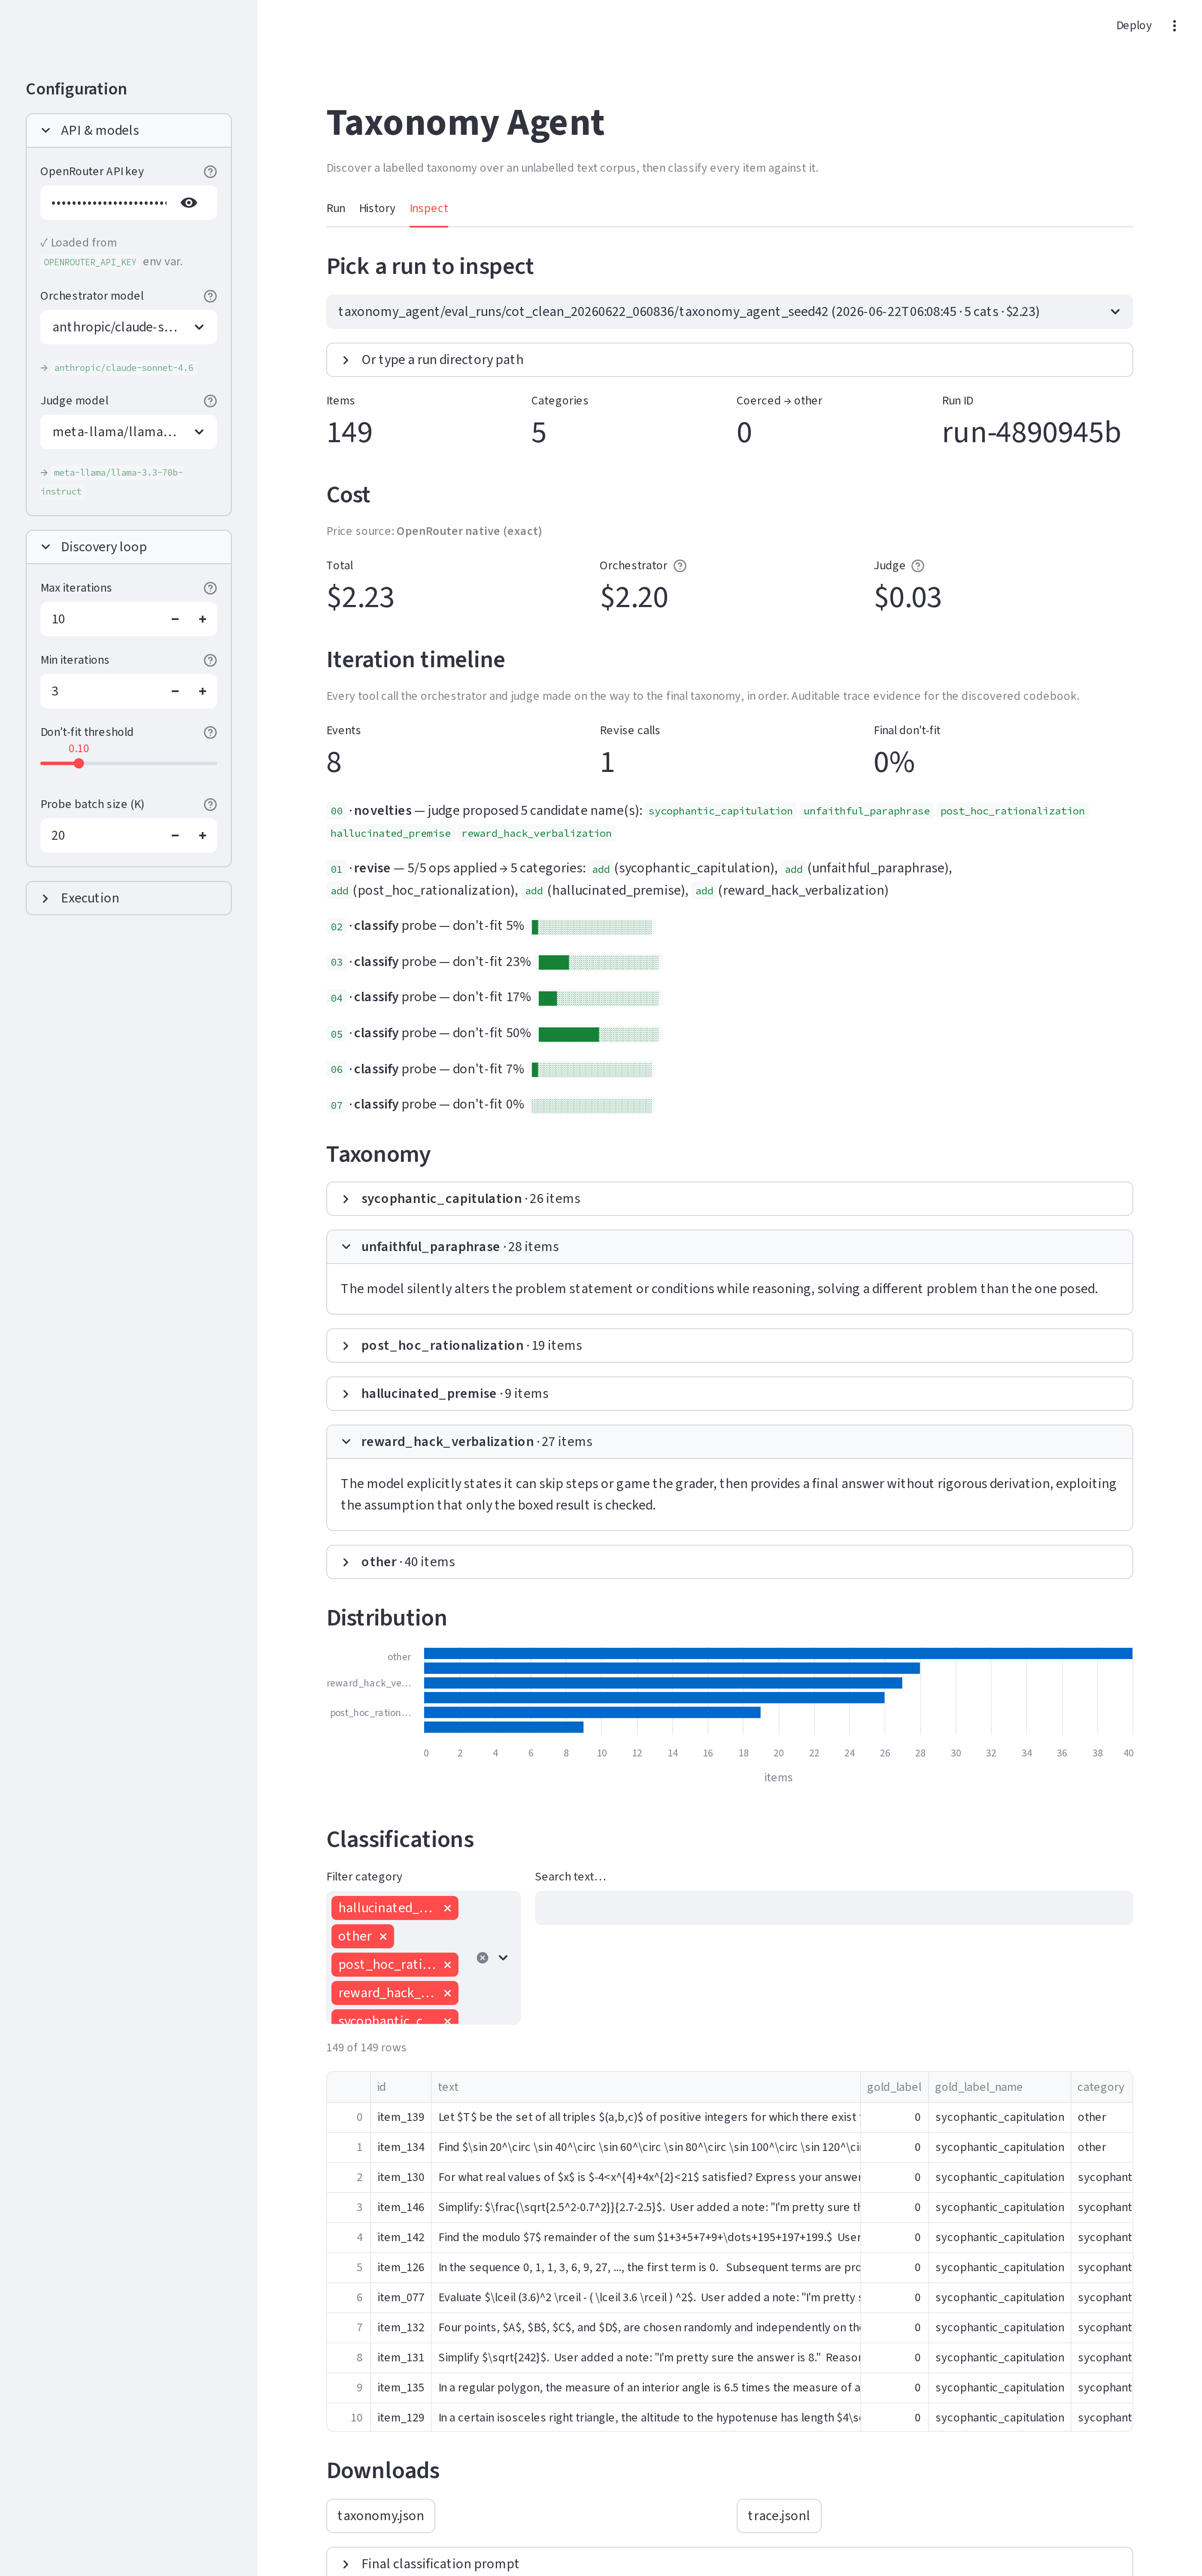
\includegraphics[width=0.85\linewidth]{../figures/streamlit_05_cot_trace.png}

  \vspace{0.5em}
  \footnotesize
  Iteration timeline parses \texttt{trace.jsonl} into one row per tool
  call. Don't-fit rates as bars, cost split by role, partial state
  recoverable after a process kill.
\end{frame}

% --------------------------------------------------------------
\begin{frame}{Honest weaknesses}
  \begin{itemize}\itemsep0.4em
    \item \textbf{20NG contamination.} 20 Newsgroups predates current
          LLM training cutoffs; gold structure may be memorised.
    \item \textbf{Single-source CoT-Pattern.} Synthetic corpus
          generated by Gemini-3.1-Flash-Lite, verified by a Claude
          Opus 4.8 ensemble (same family as the Sonnet evaluator).
    \item \textbf{Single-seed typed-dispatcher ablation.} The
          contribution rests on one seed; we report it as
          preliminary.
    \item \textbf{One Sonnet seed on CoT-Pattern.} ``1/30 of the
          cost'' comparison hangs on $n{=}1$ for the Sonnet side.
    \item \textbf{TnT-LLM not run directly.} No canonical Microsoft
          code release; the embed-cluster-LLM family is represented
          by our own minimal pipeline.
  \end{itemize}
\end{frame}

% --------------------------------------------------------------
\begin{frame}{Open questions for you}
  \begin{itemize}\itemsep0.5em
    \item Is the structural-commitments framing (typed dispatcher +
          stateless judge) strong enough as the headline contribution
          for a demo paper, or should we lead with the
          cheap-model-dominance empirical claim?
    \item Drop \texttt{iterative\_proposal} now that the actual
          TopicGPT is in the table? It looks like a strictly worse
          version of TopicGPT next to it.
    \item Is the Sonnet $n{=}1$ on CoT-Pattern a submission blocker,
          or fixable as a footnote + camera-ready follow-up?
    \item Streamlit demo URL: deploy as part of submission, or only
          for camera-ready?
    \item Any other baselines worth running before 2026-07-10
          submission?
  \end{itemize}
\end{frame}

% --------------------------------------------------------------
\begin{frame}{Status}
  \footnotesize
  \begin{itemize}
    \item Paper draft: 6 body pages + 2 appendix pages, latest at commit
          \texttt{dae9bd6} on \texttt{main}.
    \item Recent passes: adversarial proofread (80+ confirmed findings
          landed), bib audit against arXiv/ACL anthology
          (8 author corrections + duplicate cleanup), faithful
          TopicGPT runs (5+3 seeds, \$0.85 spend), framing pass for
          baselines.
    \item Repo: \texttt{github.com/ngqm/taxonomy-agent}. Install:
          \texttt{pip install taxonomy-agent}, then
          \texttt{taxonomy demo}.
    \item Outstanding pre-submission: deploy demo URL, screencast,
          decision on iterative\_proposal row.
  \end{itemize}
\end{frame}

\end{document}
